\documentclass[12pt]{article}
\usepackage{float}

\usepackage[utf8]{inputenc}
\usepackage[T1]{fontenc}
\usepackage[french]{babel}
\usepackage{amsmath, amssymb}
\usepackage{graphicx}
\usepackage{geometry}
\usepackage{hyperref}
\geometry{margin=2.5cm}
\usepackage{titlesec}

\setlength{\parindent}{15pt}
\setlength{\parskip}{1em}



\begin{document}

% Page de titre personnalisée
\begin{titlepage}
    \centering

    
\includegraphics[width=4cm]{logo.png}\par\vspace{1cm}

    \textsc{\large Master 1 MSS}\\[1.5cm]

    % Titre du projet
    {\Huge\bfseries Processus Décisionnels de Markov\\[0.3cm]
    et Apprentissage par Renforcement\\[1cm]}

    \vfill

    \begin{flushleft}
        \textbf{Auteurs :} Lahontâa Théo, Aboukacem Elias, Zidane Zine Eddine \\
        \textbf{Encadrant :} Adrien Richou \\
    \end{flushleft}

    \vfill

    \centering
    Rapport de TER\\
    Année universitaire 2024--2025

\end{titlepage}


\tableofcontents
\newpage




\section*{Introduction}

Dans ce projet nous allons nous intéresser aux processus décisionnels Markoviens (PDM), un cadre mathématique qui permet de modéliser des prises de décision dans des environnements évoluant de manière aléatoire. L’idée générale est de représenter la situation d’un système par un état, sur lequel un agent peut agir en choisissant une action. Cette action entraîne une transition vers un nouvel état selon une certaine probabilité, et produit une récompense (ou un coût). L’objectif est de déterminer une politique de décision, c’est-à-dire une règle qui indique quelle action choisir à chaque instant, de manière à optimiser un critère global (souvent, la somme des récompenses espérées).

Dans une première partie, nous étudions les aspects théoriques du modèle. À partir du chapitre 1 de l’ouvrage Processus Décisionnels de Markov en Intelligence Artificielle (groupe PDMIA), nous introduisons formellement les PDM : définition des objets fondamentaux (états, actions, probabilités de transition, fonction de récompense), types de politiques, fonctions de valeur, et différents critères d’évaluation (horizon fini, actualisé, total, moyen). L’objectif est de comprendre précisément les outils qui permettent de formuler et d’analyser ce type de problèmes.

La seconde partie du projet est pratique. Elle consiste à mettre en œuvre certains algorithmes de résolution des PDM dans des environnements simulés, en utilisant la bibliothèque Python Gymnasium. Nous étudierons notamment les méthodes classiques comme value iteration et policy iteration, en observant comment elles permettent à un agent d'apprendre à se comporter de façon optimale dans un cadre donné.

L’ensemble du projet vise ainsi à se familiariser avec les principes de base de l'apprentissage par renforcement puis établir un lien entre la théorie et la pratique en formalisant rigoureusement des situations de décision séquentielle, puis les traduire en simulations concrètes permettant d’observer et d’analyser les résultats obtenus.

 \newpage

\section{Modélisation des processus décisionnels de Markov}

\subsection{Cadre général}

Les processus décisionnels de Markov (PDM) constituent un cadre mathématique pour modéliser des situations où un agent prend des décisions successives dans un environnement incertain. À chaque instant, l’agent observe un état du système, choisit une action, et reçoit une récompense dépendant de cette action et de l’état. L’état du système évolue ensuite de manière aléatoire selon une dynamique probabiliste influencée par l’action choisie.

Ce type de modélisation intervient dans de nombreux domaines : planification, robotique, contrôle optimal, ou encore apprentissage automatique. Dans ce projet, les PDM serviront de base théorique à l’apprentissage par renforcement, dont ils constituent le modèle sous-jacent.

\subsection{Définition}

Un PDM est défini par un quintuplet \((S, A, T, p, r)\) où :
\begin{itemize}
    \item \(S\) est l’espace des états. Il décrit l’ensemble des situations possibles du système.
    \item \(A\) est l’espace des actions disponibles pour l’agent.
    \item \(T\) est l’ensemble des instants de décision. On suppose ici \(T = \mathbb{N}\) (temps discret), éventuellement borné (horizon fini) ou infini.
    \item \(p : S \times A \times S \rightarrow [0,1]\) est la fonction de transition, telle que \(p(s'|s,a)\) donne la probabilité que le système passe de l’état \(s\) à l’état \(s'\) après l’action \(a\).
    \item \(r : S \times A \rightarrow \mathbb{R}\) est la fonction de récompense, qui associe à chaque paire \((s,a)\) une récompense attendue \(r(s,a)\).
\end{itemize}

Une représentation alternative permet aussi d’utiliser une fonction \(r(s, a, s')\) définie sur les transitions, auquel cas on définit la récompense moyenne :
\[
\bar{r}(s, a) = \sum_{s' \in S} p(s'|s,a) \cdot r(s,a,s').
\]

\subsection{Hypothèses usuelles}

Dans le cadre de ce projet, nous considérons les hypothèses classiques suivantes :
\begin{itemize}
    \item \textbf{Hypothèse de Markov} : la dynamique ne dépend que de l’état courant et de l’action, pas de l’historique. Formellement :
    \[
    \mathbb{P}(s_{t+1} = s' \mid h_t, a_t) = \mathbb{P}(s_{t+1} = s' \mid s_t, a_t),
    \]
    où \(h_t\) est l’historique jusqu’au temps \(t\).
\vspace{0.5em}
    \item \textbf{Stationnarité} : les probabilités de transition et la fonction de récompense ne varient pas avec le temps.
\vspace{0.5em}
    \item \textbf{Récompenses bornées} : on suppose que \(r(s,a)\) est bornée pour tout \((s,a)\), ce qui garantit l’existence des espérances intervenant dans les critères de performance.
\end{itemize}

\section{Politiques, critères de performance et fonctions de valeur}

\subsection{Définitions des politiques}

Une politique (ou règle de décision) est une règle qui spécifie l’action à effectuer à chaque instant de décision. Elle peut être :

\begin{itemize}
    \item \textbf{Déterministe} : une fonction \(\pi : S \to A\), qui associe à chaque état une action.
\vspace{0.5em}
    \item \textbf{Aléatoire} : une fonction \(\pi : S \to \mathcal{P}(A)\), qui donne une distribution de probabilité sur les actions possibles à partir d’un état donné.
\end{itemize}

On distingue également :

\begin{itemize}
    \item \textbf{Politiques stationnaires} : indépendantes du temps, c’est-à-dire que la règle de décision ne change pas selon l’instant \(t\).
\vspace{0.5em}
    \item \textbf{Politiques non-stationnaires} : pouvant varier au cours du temps, par exemple \(\pi_t : S \to A\) à chaque instant \(t\).
    
\end{itemize}

Enfin, une politique peut dépendre de l’historique complet \(h_t = (s_0, a_0, s_1, a_1, \dots, s_t)\), on parle alors de \textbf{politique histoire-dépendante}. Cependant, sous l’hypothèse de Markov, on peut démontrer que toute politique histoire-dépendante peut être remplacée par une politique \textbf{markovienne} (dépendant uniquement de l’état courant) ayant la même fonction de valeur. Cela justifie que l’on restreint généralement l’étude aux politiques markoviennes.

\subsection{Critères de performance et fonctions de valeur}

Le choix d’un critère de performance permet de quantifier la performance d’une politique \(\pi\) en fonction de la récompense attendue lorsque cette politique est suivie à partir d’un état donné. Chaque critère correspond à une manière d’agréger les récompenses dans le temps, et donne lieu à une fonction associée que l’on appelle fonction de valeur.

Cette fonction permet de comparer différentes politiques. Les expressions suivantes présentent les principales variantes utilisées.

\begin{itemize}
    \item \textbf{Critère fini} : pour un entier \(N > 0\), on considère la somme des récompenses sur les \(N\) premiers instants :
    \[
    V^\pi_N(s) = \mathbb{E}_\pi \left[ \sum_{t=0}^{N-1} r(s_t, a_t) \,\middle|\, s_0 = s \right]
    \]
    Ce critère est adapté aux situations où l’horizon temporel est déterminé à l’avance.
\vspace{0.5em}

    \item \textbf{Critère \(\gamma\)-pondéré} :
    \[
    V^\pi_\gamma(s) = \mathbb{E}_\pi \left[ \sum_{t=0}^{\infty} \gamma^t r(s_t, a_t) \,\middle|\, s_0 = s \right], \quad \gamma \in (0,1)
    \]
    Les récompenses futures sont pondérées par un facteur \(\gamma\). Ce critère assure la convergence de la série si les récompenses sont bornées.
\vspace{0.5em}
    \item \textbf{Critère total } :
    \[
    V^\pi(s) = \mathbb{E}_\pi \left[ \sum_{t=0}^{\infty} r(s_t, a_t) \,\middle|\, s_0 = s \right]
    \]
    Il mesure la récompense cumulée totale. Son usage nécessite des hypothèses supplémentaires pour garantir l’existence de l’espérance.
\vspace{0.5em}
    \item \textbf{Critère moyen} :
    \[
    V^\pi(s) = \limsup_{n \to \infty} \frac{1}{n} \mathbb{E}_\pi \left[ \sum_{t=0}^{n-1} r(s_t, a_t) \,\middle|\, s_0 = s \right]
    \]
    Ce critère correspond à la récompense moyenne par unité de temps. Il est utilisé dans les situations où le processus est supposé infini sans horizon fixe.
\end{itemize}

Les fonctions \(V^\pi(s)\), \(V^\pi_\gamma(s)\), \(g^\pi(s)\), etc., définies par ces critères, sont les quantités utilisées pour évaluer et comparer les politiques.



\subsection{Politiques optimales}

Une politique \(\pi^*\) est dite optimale si elle maximise la fonction de valeur parmi toutes les politiques admissibles, pour tout état :
\[
V^{\pi^*}(s) = \sup_{\pi} V^\pi(s), \quad \forall s \in S
\]
On note alors \(V^*(s)\) la fonction de valeur optimale définie par :
\[
V^*(s) = \sup_{\pi} V^\pi(s)
\]

L’existence d’une politique optimale dépend du critère utilisé et des propriétés du modèle. Par exemple, dans le cas du critère \(\gamma\)-pondéré, si les récompenses sont bornées et si les espaces d’états et d’actions sont finis, alors il existe une politique stationnaire déterministe optimale. Dans d’autres cas (critère total, critère moyen, espaces infinis, etc.), des hypothèses supplémentaires peuvent être nécessaires, et la politique optimale peut ne pas être stationnaire ou déterministe.

La recherche d’une politique optimale constitue l’objectif des méthodes étudiées dans la suite du projet.

\section{Étude d’un environnement simple : labyrinthe déterministe}


Avant d’envisager des implémentations informatiques, on propose dans ce chapitre d’illustrer concrètement l’application du formalisme des processus décisionnels de Markov sur un exemple élémentaire : un labyrinthe de dimension $5 \times 6$, représenté à la figure~\ref{fig:labyrinthe}. Cet environnement est entièrement déterministe : à chaque étape, l’action choisie détermine de manière certaine la transition vers un nouvel état, sauf lorsqu’elle est bloquée par un mur ou par les limites du labyrinthe.

\begin{figure}[h]
    \centering
    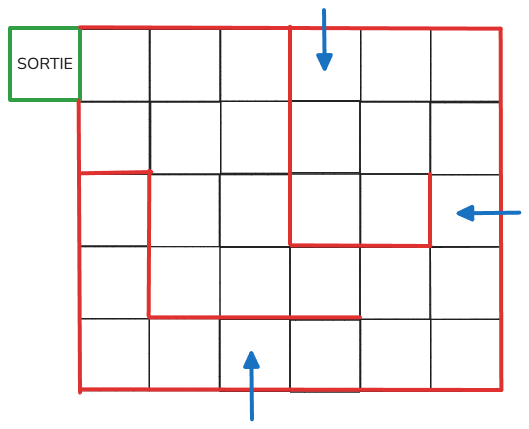
\includegraphics[width=0.6\textwidth]{labyrinthevierge.png}
    \caption{Labyrinthe utilisé pour illustrer des trajectoires simples. Les flèches bleues indiquent les positions d’entrée, la sortie est encadrée en vert.}
    \label{fig:labyrinthe}
\end{figure}

\subsection{Exploration intuitive du labyrinthe}

On considère ici différentes politiques simples, définies comme des règles fixes s’appliquant à chaque décision.

\begin{itemize}
    \item \textbf{Politique 1 : aller toujours à droite.}  
    L’agent applique l’action \texttt{droite} à chaque étape, tant que cela est possible. Cette politique se révèle rapidement inefficace, car la présence de murs ou de bordures bloque très vite la progression, quelle que soit l’entrée choisie.
\vspace{0.5em}
    \item \textbf{Politique 2 : suivre un ordre fixe de priorités (droite > bas > gauche > haut).}  
    À chaque étape, l’agent choisit la première direction possible parmi cette liste, en évitant les directions bloquées. Cette politique est plus efficace que la précédente, et permet à certains agents d’atteindre la sortie, mais reste sous-optimale car elle ne tient pas compte de la structure globale du labyrinthe.
\vspace{0.5em}
    \item \textbf{Politique 3 : éviter les cases déjà visitées.}  
    L’agent mémorise les cases déjà explorées et refuse de les revisiter. Lorsqu’il a plusieurs choix possibles, il choisit celui qui ne mène pas à une boucle. Cette stratégie permet d’éviter les cycles inutiles, mais impose une mémoire de l’historique.
\end{itemize}

\vspace{0.5em}

Remarque :
La politique 3, bien que naturelle dans un contexte de navigation, n’est pas une politique markovienne au sens strict : sa décision dépend de l’historique des états visités. Elle relève donc de la classe des politiques histoire-dépendantes. Pour la prendre en compte dans le cadre formel des PDM, il faudrait enrichir l’espace d’états pour inclure, par exemple, l’ensemble des positions déjà explorées.

\subsection{Modélisation du labyrinthe comme processus décisionnel de Markov}


On reprend ici l’environnement présenté précédemment et on le formalise comme un processus décisionnel de Markov. L’objectif est d’en définir les composantes principales selon le formalisme standard : ensemble des états, ensemble des actions, dynamique de transition et fonction de récompense.

\paragraph{Ensemble des états.}
On considère un labyrinthe de dimension $L \times C$ avec $L = 5$ et $C = 6$. L’ensemble des états est constitué des cases accessibles de la grille, ainsi que d’un état terminal d’arrivée noté $s^*$ :
\[
S = \left\{ (i,j) \;\middle|\; 1 \leq i \leq L,\; 1 \leq j \leq C \right\} \cup \{s^*\}
\]

\paragraph{Ensemble des actions.}
L’ensemble des actions disponibles en chaque état est donné par :
\[
A = \{\uparrow, \downarrow, \leftarrow, \rightarrow\}
\]
Ces actions correspondent respectivement aux déplacements vers le haut, le bas, la gauche et la droite.

\paragraph{Dynamique de transition.}
La fonction de transition $p(s' \mid s, a)$ est définie de manière déterministe, selon les règles suivantes :
\[
p(s' \mid s, a) =
\begin{cases}
1 & \text{si } s = s' = s^* \\
1 & \text{si } a \text{ permet de passer de } s \text{ à } s' \text{ en un coup, sans mur entre les deux} \\
1 & \text{si } s = s' \text{ et l'action } a \text{ mène à un mur ou en dehors du labyrinthe} \\
0 & \text{sinon}
\end{cases}
\]

Par convention, on considère que l’action \(\leftarrow\) effectuée depuis la case \((1,1)\) permet une transition vers l’état terminal \(s^*\), interprété comme la sortie du labyrinthe.

La structure des murs et des déplacements valides est déterminée par le labyrinthe représenté à la figure~\ref{fig:labyrinthe}. Toute tentative de déplacement à travers un mur ou en dehors de la grille est considérée comme invalide et laisse l’état inchangé.

\paragraph{Fonction de récompense.}
La fonction de récompense \(r : S \times A \to \mathbb{R}\) est définie par :
\[
r(s,a) =
\begin{cases}
R & \text{si } s = (1,1) \text{ et } a = \leftarrow \\
0 & \text{si } s = s^* \\
-1 & \text{sinon}
\end{cases}
\]

La récompense positive \(R\) est obtenue uniquement lorsque l’agent choisit de sortir du labyrinthe via la case \((1,1)\). Toutes les autres transitions ont un coût unitaire, sauf lorsque l’agent reste dans l’état terminal.

La valeur de \(R\) doit être choisie strictement supérieure au nombre maximal de déplacements possibles dans le labyrinthe, soit ici \(R > 30\), afin que la sortie soit préférée à toute trajectoire pénalisante, même si elle est longue.

\subsection{Résolution pour le critère fini}

On suppose dans cette partie que l’agent dispose d’un nombre fixé d’étapes, noté \(N\), pour maximiser la récompense accumulée à partir d’un état initial donné. Le critère utilisé est donc :
\[
V^\pi_N(s) = \mathbb{E}_\pi \left[ \sum_{t=0}^{N-1} r(s_t, a_t) \,\middle|\, s_0 = s \right]
\]
Dans le cas déterministe considéré ici, cette quantité peut être calculée de manière exacte par récurrence sur l’horizon.

\paragraph{Fonction de valeur au rang 1 (\(V_1\)).}

La fonction \(V_1(s)\) correspond à la récompense obtenue en un seul déplacement à partir de l’état \(s\). Elle est donnée par :
\[
V_1(s) = \max_{a \in A} r(s,a)
\]

Dans notre modèle :
- toutes les actions donnent une récompense \(-1\), sauf
- l’action \(\leftarrow\) depuis \((1,1)\), qui donne \(R\), et
- l’état \(s^*\), qui donne 0.

Ainsi, la fonction \(V_1\) est égale à \(R\) en \((1,1)\), à 0 en \(s^*\), et à \(-1\) ailleurs.

\vspace{1em}
\begin{figure}[h]
    \centering
    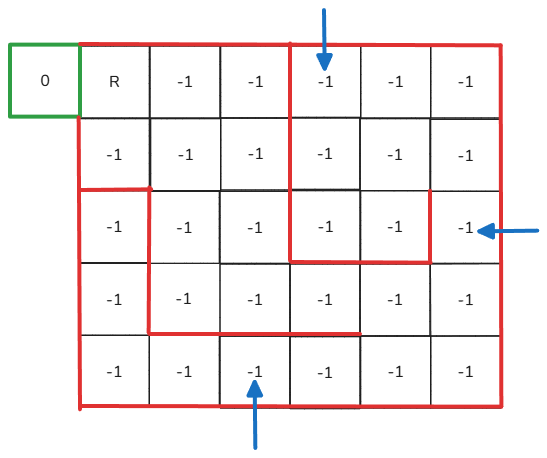
\includegraphics[width=0.6\textwidth]{labyrinthev1.png}
    \caption{Valeur de la fonction \(V_1\) : récompense maximale en un seul déplacement.}
    \label{fig:V1}
\end{figure}

\paragraph{Formule de récurrence.}

De manière générale, dans le cadre d’un processus décisionnel de Markov à horizon fini, la fonction de valeur optimale peut être construite récursivement selon la relation suivante :
\[
V_{n+1}^{*}(s) = \max_{a \in A} \left[ r(s,a) + \sum_{s' \in S} p(s' \mid s, a) \cdot V_n^{*}(s') \right]
\]

Dans notre cas particulier, le système est entièrement déterministe : pour chaque état \(s\) et action \(a\), il existe un unique état \(s' = f(s,a)\) tel que \(p(s' \mid s, a) = 1\), et les autres transitions ont une probabilité nulle. Par conséquent, la formule se simplifie en :
\[
V_{n+1}(s) = \max_{a \in A} \left[ r(s,a) + V_n(f(s,a)) \right]
\]
Cette version est utilisée dans la suite pour construire itérativement la fonction de valeur pour le critère fini.


\paragraph{Fonction de valeur au rang 2 (\(V_2\)).}

À partir de \(V_1\), on calcule \(V_2(s)\) pour chaque état \(s\), en considérant tous les déplacements possibles et en maximisant la somme de la récompense immédiate et de la valeur obtenue à l’étape suivante.

\vspace{1em}
\begin{figure}[h]
    \centering
    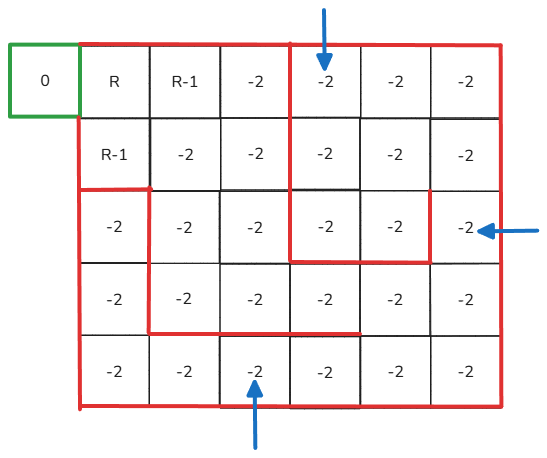
\includegraphics[width=0.6\textwidth]{labyrinthev2.png}
    \caption{Valeur de la fonction \(V_2\) : récompense maximale en deux déplacements.}
    \label{fig:V2}
\end{figure}

\vspace{0.5em}
\noindent Ce processus peut être itéré jusqu’à l’horizon choisi \(N\), ce qui permet de construire la fonction \(V_N\) et, par extension, d’en déduire une politique optimale par rétropropagation.

\begin{figure}[H]
    \centering
    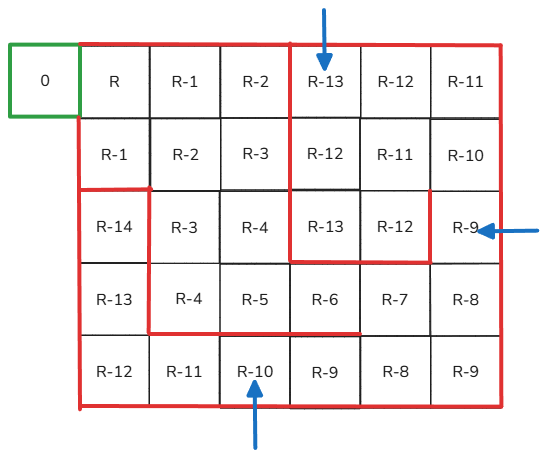
\includegraphics[width=0.6\textwidth]{labyrintheVn.png}
    \caption{Valeur de la fonction \(V_N\) pour un horizon fixé.}
    \label{fig:Vn}
\end{figure}



À partir de la fonction de valeur optimale \(V_N^*\), il est possible de déterminer la politique optimale \(\pi^*\) associée. Celle-ci consiste, pour chaque état \(s\), à choisir l’action \(a \in A\) qui maximise la somme de la récompense immédiate et de la valeur atteignable à l’étape suivante :
\[
\pi^*(s) \in \arg\max_{a \in A} \left[ r(s,a) + V_{N-1}^*(f(s,a)) \right]
\]
où \(f(s,a)\) désigne l’état atteint à partir de \(s\) en appliquant l’action \(a\).

Dans notre environnement déterministe, cette politique peut être construite de manière explicite en suivant l’évolution de la fonction de valeur à rebours : à chaque état, on choisit l’action qui permet d’atteindre un état de plus grande valeur (c’est-à-dire plus proche de la sortie), en minimisant le coût cumulé.

\vspace{1em}
\begin{figure}[H]
    \centering
    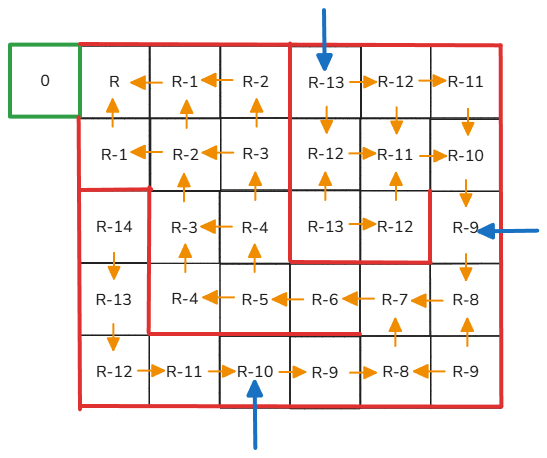
\includegraphics[width=0.6\textwidth]{politiquelab.png}
    \caption{Politique optimale associée à la fonction \(V_N^*\) pour un horizon donné.}
    \label{fig:policyN}
\end{figure}

On obtient ainsi une stratégie qui guide l’agent depuis n’importe quelle position accessible vers la sortie de manière optimale, dans la limite de l’horizon \(N\) fixé.


En posant \(d\) la distance d’un état \(s\) à la sortie, on observe que la fonction de valeur optimale vérifie la relation suivante :
\[
V_N(s) = R - d + 1.
\]
La valeur décroît donc linéairement avec la distance à la sortie.

\subsection{Résolution pour le critère $\gamma$-pondéré}

Dans le cas du critère $\gamma$-pondéré, on s'intéresse à une somme de récompenses actualisées cette fois sur un horizon infini, avec un facteur $0 \leq \gamma < 1$ qui diminue le poids des récompenses futures. La fonction de valeur associée à une politique $\pi$ est définie comme la solution de l'équation :
\[
\forall s \in S \quad V(s) = r_\pi(s) + \gamma \sum_{s' \in S} P_{\pi, s, s'} V(s').
\]
Cette équation peut être interprétée comme la recherche d’un point fixe de l’opérateur de Bellman $T_\pi$, défini par $T_\pi V(s) = r_\pi(s) + \gamma \sum_{s'} P_{\pi, s, s'} V(s')$.


Un des moyens pour approcher cette solution est donc d'introduire une suite $(V_n)_{n \geq 0}$ définie par récurrence :
\[
V_{n+1}(s) = r_\pi(s) + \gamma \sum_{s' \in S} P_{\pi, s, s'} V_n(s'), \quad \text{avec } V_0 \in \mathbb{R}^{|S|}.
\]
Lorsque $\gamma < 1$, cette suite converge vers l’unique point fixe de l’opérateur $T_\pi$, qui est précisément la fonction de valeur $V^\pi_\gamma$.


En utilisant la même méthode de récurrence que pour le critère fini, on peut approcher la fonction de valeur associée au critère $\gamma$-pondéré. Dans le cas du labyrinthe déterministe, une résolution manuelle cnous permet d'obtenir une formule générale pour ce critère. En posant \(d\) la distance d’un état \(s\) à la sortie, on obtient :
\[
V(s) = \sum_{k=0}^{d-1} \gamma^k (-1) + \gamma^d R = -\frac{1 - \gamma^d}{1 - \gamma} + \gamma^d R
\]

Le premier terme correspond aux pénalités de chaque déplacement, et le second terme à la récompense reçue en atteignant la sortie.

En maximisant, pour chaque état, la fonction de valeur  sous le critère $\gamma$-pondéré, on obtient la même politique optimale que dans le cas du critère fini. Cela semble logique et  s’explique par le fait que, dans un environnement déterministe, les deux approches vont privilégier les trajectoires les plus courtes vers la sortie.

\section{Étude d’un environnement aléatoire : labyrinthe avec téléporteur}

Dans cette dernière partie théorique, nous allons reprendre le labyrinthe étudié précédemment, mais en introduisant un élément d’aléa : un téléporteur. Lorsque l’agent passe sur la case téléporteur, il est automatiquement transporté vers l’état juste avant la sortie. Ce changement modifie la dynamique du système et impose une modélisation probabiliste de la transition.

L’objectif ici est d’analyser l’impact de cette modification sur la fonction de valeur et sur la politique optimale, en comparant avec les résultats obtenus dans le cas déterministe.

Voici le labyrinthe considéré, identique au précédent à l’exception d’une case téléporteur notée \(T\), qui envoie l’agent directement sur la case notée \(T'\) juste avant la sortie.


\begin{figure}[H]
    \centering
    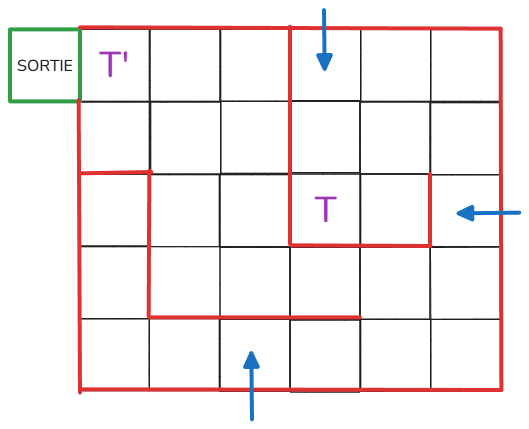
\includegraphics[width=0.6\textwidth]{labyrinthetéléporteur.png}
    \caption{Labyrinthe avec téléporteur}
    \label{fig:labyrinthe_teleporteur}
\end{figure}

\subsection{Adaptation du processus décisionnel de Markov}

L’ensemble des états et des actions reste identique à celui du modèle déterministe. La fonction de récompense \(r\) n’est pas affectée par l’introduction du téléporteur, et s’écrit toujours(nous avons juste renommé la case (1,1) en T') :

\[
r(s, a) =
\begin{cases}
R & \text{si } s = T' \text{ et } a = \leftarrow \\
0 & \text{si } s = s^* \\
-1 & \text{sinon}
\end{cases}
\]


Seule la fonction de transition \(p(s' \mid s, a)\) est modifiée pour intégrer l’effet du téléporteur.
La fonction de transition $p(s' \mid s, a)$ est donc redéfinie comme :

\[
p(s' \mid s, a) = 
\begin{cases}
1 & \text{si } s = s' = s^* \\
1 & \text{si } a \text{ permet de passer de } s \text{ à } s' \text{ en un coup, sans mur entre les deux, et } s' \neq T \\
p & \text{si } s' = T' \text{ et } (a \text{ permet d’aller de } s \text{ à } T \text{ ou } s = T \text{ et } a \text{ mène à un mur}) \\
1 - p & \text{si } s' = T \text{ et } (a \text{ permet d’aller de } s \text{ à } T \text{ ou } s = T \text{ et } a \text{ mène à un mur}) \\
1 & \text{ si } s = s' \text{ et } a \text{ mène à un mur, ou si } s \neq T \\
0 & \text{sinon}
\end{cases}
\]

La dynamique reste identique à celle du modèle déterministe pour toutes les transitions ne faisant pas intervenir la case téléporteur T ou la case avant la sortie T'.

\subsection{Résolution avec critère fini}

Nous allons calculer par récurrence la fonction de valeur optimale associée au critère fini, en présence du téléporteur. À chaque étape \(n\), on détermine \(V_n(s)\) pour toutes les cases du labyrinthe, afin d’analyser comment la dynamique évolue en fonction de la probabilité \(p\).


Ce cadre permet de mettre en évidence l’existence de deux types de contributions à la valeur d’un état : une contribution classique liée au chemin direct vers la sortie, et une contribution probabiliste liée au passage par le téléporteur. Une fois la fonction de valeur établie, on pourra en déduire la politique optimale  et l’analyser en fonction de la probabilité \(p\).

\paragraph{Fonction de valeur au rang 1}

À l’étape \(n = 1\), seule la case située juste avant la sortie permet d’atteindre \(s^*\) en un coup. C’est la seule situation où la récompense \(R\) peut être obtenue à ce rang. Toutes les autres actions, y compris celles menant au téléporteur ou restant sur la case \(T\), ne permettent pas d’atteindre la sortie à cette étape et ne rapportent donc aucune récompense. L’agent ne subit alors que le coût de l’action effectuée.

On obtient donc :
\[
V_1(s) =
\begin{cases}
R & \text{si } s \text{ mène directement à } s^* \\
-1 & \text{sinon}
\end{cases}
\]


\begin{figure}[H]
    \centering
    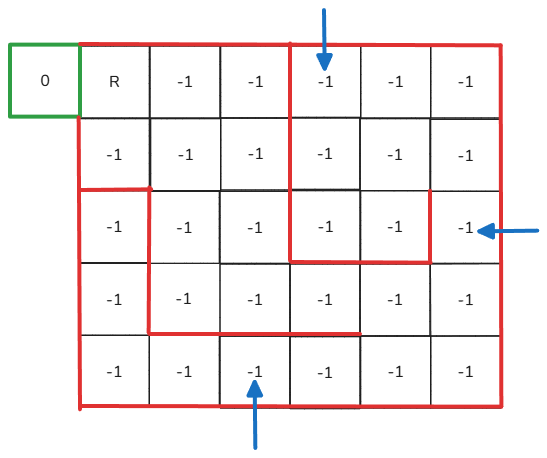
\includegraphics[width=0.55\textwidth]{labyrinthev1.png}
    \caption{Fonction de valeur \(V_1\) dans le labyrinthe avec téléporteur}
\end{figure}

\paragraph{Calcul de \(V_2\) dans le cas du téléporteur}

Pour mieux comprendre le rôle de la probabilité \(p\), on calcule ici \(V_2(s)\) pour une case \(s\) adjacente à la case téléporteur \(T\). L’agent choisit une action qui le mène sur \(T\). Cette action coûte \(-1\), puis le téléporteur agit immédiatement après l’arrivée.

On a donc ces 2 cas :
\begin{itemize}
    \item avec probabilité \(p\), l’agent est téléporté sur \(T'\), et peut ensuite atteindre la sortie au rang suivant. Comme \(V_1(T') = R\), cette trajectoire apporte un gain de \(p \cdot R\) ;
    \item avec probabilité \(1 - p\), l’agent reste sur \(T\). Il ne peut pas atteindre la sortie au rang suivant et \(V_1(T) = -1\).
\end{itemize}

On en déduit :
\[
V_2(s) = -1 + p \cdot V_1(T') + (1 - p) \cdot V_1(T) = -1 + Rp + (-1)(1 - p)
= Rp + p - 2
\]

Ce calcul met en évidence la forme typique des fonctions de valeur associées à un chemin passant par le téléporteur. Il servira de base pour généraliser au rang \(n\) dans le paragraphe suivant.


\paragraph{Fonction de valeur au rang \(n\)} 
On reprend la formule générale de la fonction de valeur au rang \(n\), donnée par :
\[
V_{n+1}(s) = \max_{a \in A} \left[ r(s,a) + \sum_{s' \in S} p(s' \mid s, a) \cdot V_n(s') \right]
\]

Dans le cas d’un chemin déterministe vers la sortie, cette expression peut être simplifiée comme précédemment. En posant \(d\) la distance à la sortie, et en supposant que l’agent suit le chemin optimal sans aléa, on retrouve :
\[
V_n^{(\text{direct})}(s) = R - d + 1
\]

\begin{figure}[H]
    \centering
    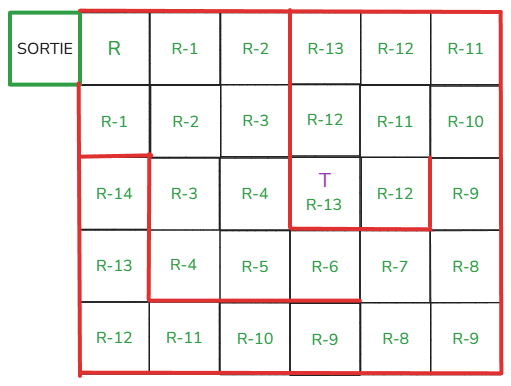
\includegraphics[width=0.55\textwidth]{labyrinthesortie1.png}
    \caption{Fonction de valeur sans passer par le téléporteur}
\end{figure}

En revanche, pour un chemin passant par le téléporteur, il faut prendre en compte l’aléa induit par la probabilité \(p\). On se place dans le cas où l’agent part d’un état \(s\), atteint la case téléporteur \(T\) en \(d_T\) étapes, puis subit l’effet probabiliste du téléporteur.

Chaque déplacement coûte \(-1\), donc atteindre \(T\) depuis \(s\) engendre un coût total de \(-d_T\). Une fois sur \(T\), deux cas sont possibles :
\begin{itemize}
    \item avec probabilité \(p\), l’agent est téléporté vers la case \(T'\), puis entre dans la case sortie et reçoit la récompense \(R\) ;
    \item avec probabilité \(1 - p\), l’agent reste sur \(T\), ne progresse pas, et subit un coût supplémentaire de \(-1\) à ce rang.
\end{itemize} 

La valeur espérée à partir de \(s\) est donc :
\[
V_n^{(\text{téléporteur})}(s) = -d_T + \left[pR + (1 - p)(-1)\right] = Rp + p - 1 - d_T
\]

Dans le cas où l'agent est déjà sur le téléporteur (par exemple si il ne s'est pas déclenché à l'étape précédente), alors il si il fait une action qui mène à un mur, il reste sur le téléporteur et a de nouveau une probabilité p de l'activer. Dans ce cas, on a donc \(d_T = 1\), et la formule donne :
\[
V_n(T) = Rp + p - 2
\]

\begin{figure}[H]
    \centering
    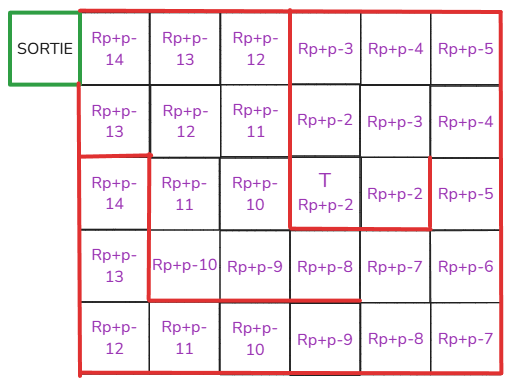
\includegraphics[width=0.4\textwidth]{labyrinthesortie2.png}
    \caption{Fonction de valeur via le téléporteur}
\end{figure}

La fonction de valeur \(V_n(s)\) est donnée par le maximum entre les deux contributions possibles : celle du chemin direct vers la sortie, et celle du chemin passant par le téléporteur. En posant \(d(s)\) la distance de l’état \(s\) à la sortie, et \(d_T(s)\) sa distance à la case téléporteur, on a :

\[
V_n(s) = \max \left( R - d(s) + 1,\; Rp + p - 1 - d_T(s) \right)
\]

Pour déterminer à partir de quelle valeur de \(p\) le chemin passant par le téléporteur devient préférable, on résout l’équation d’égalité entre les deux expressions :

\[
R - d(s) + 1 = Rp + p - 1 - d_T(s)
\]

Ce qui nous donne, après simplification :

\[
p^*(s) = \frac{R - d(s) + d_T(s) + 2}{R + 1}
\]

Cette valeur correspond à la probabilité minimale pour que le téléporteur devienne une meilleure option que le chemin direct, pour l’état \(s\) considéré.

Cependant, cette expression n’a de sens que si \(d(s) > d_T(s)\). En effet, si \(d(s) \leq d_T(s)\), alors on obtient \(p^*(s) > 1\), ce qui est impossible pour une probabilité. Cela semble logique car si l’agent est plus proche de la sortie que du téléporteur, il sera toujours préférable de s’y diriger directement, quelle que soit la valeur de \(p\).

\paragraph{Analyse de la politique optimale en fonction de \(p\)}

Pour chaque état \(s\) du labyrinthe, on peut calculer la valeur \(p^*(s)\) donnée par :

\[
p^*(s) = \frac{R - d(s) + d_T(s) + 2}{R + 1}
\]

Cette quantité correspond à la probabilité minimale que doit avoir le téléporteur pour que la politique optimale choisisse de passer par celui-ci plutôt que de suivre le chemin direct vers la sortie. Autrement dit, si \(p > p^*(s)\), alors le chemin passant par le téléporteur devient optimal à partir de l’état \(s\) ; sinon, l’agent aura intérêt à se diriger directement vers la sortie.

On peut ainsi représenter visuellement, pour chaque case du labyrinthe, la valeur seuil \(p^*(s)\). Cela permet de comprendre comment la position dans l’espace influence la stratégie optimale selon la valeur de \(p\). 

Pour ce calcul, il est nécessaire de fixer une valeur de \(R\), la récompense reçue à l’arrivée dans la case de sortie, car \(p^*(s)\) en dépend directement. Par exemple, on va fixer \(R = 50\) et on calcule les valeurs \(p^*_R(s)\) associées à chaque case du labyrinthe.



\begin{figure}[H]
    \centering
    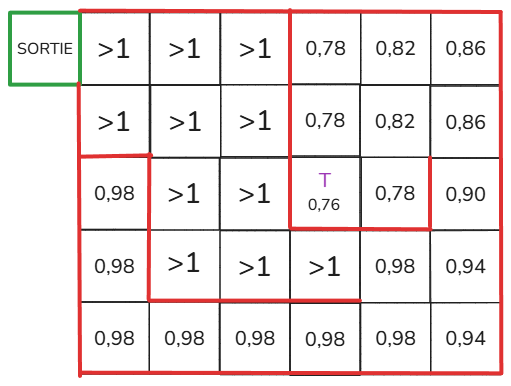
\includegraphics[width=0.5\textwidth]{labyrinthep.png}
    \caption{Valeurs de \(p^*(s)\) pour R=50}
\end{figure}

Par exemple, si on fixe \(p = 0{,}9\), alors la politique optimale consistera à se diriger vers le téléporteur uniquement à partir des cases où \(p^*(s) > 0{,}9\), et vers la sortie directe ailleurs. 

Même si les valeurs de \(p^*(s)\) peuvent sembler élevées, cela s'explique par le fait que la politique optimale se base sur l'espérance : elle ne cherche pas le scénario le plus probable, mais le gain moyen à long terme. Par exemple, avec \(p = 0{,}6\), il est peu probable que l'agent échoue plusieurs fois de suite à se téléporter, mais la fonction de valeur tient compte du coût cumulé de ces échecs s'ils se produisent. Enfin, les seuils \(p^*\) sont d'autant plus élevés ici que la récompense \(R\) a été fixée à une valeur importante, ce qui favorise le chemin direct, dont la récompense est garantie.


Pour conclure cette partie, nous avons vérifié expérimentalement nos résultats en implémentant un algorithme de Q-learning. En fixant les mêmes paramètres \(R\) et \(p\) que dans l’analyse théorique, et après une vingtaine d’épisodes dans l’environnement, nous allons voir si l’agent apprend une politique optimale qui s’aligne avec celle obtenue analytiquement à partir de la fonction de valeur.

\section{Apprentissage par renforcement}

Jusqu’ici, nous avons supposé que l’environnement était entièrement connu : probabilités de transition, fonction de récompense, etc. Dans cette dernière partie, nous nous plaçons dans un cadre plus réaliste, où l’agent ne connaît pas le modèle à l’avance. Il apprend uniquement en intéragissant avec l’environnement. C’est le principe de l’apprentissage par renforcement.

\subsection{Présentation du Q-learning}

L’objectif reste le même : apprendre une politique optimale qui maximise la récompense cumulée mais cette fois, l’agent découvre l’environnement au fur et à mesure, en explorant les états et en testant des actions.

L’algorithme que nous allons utiliser est le Q-learning, qui se base sur l’approximation d’une fonction de valeur d’action \(Q(s, a)\). Cette fonction a pour but d'estimer la valeur d’un couple \((s,a)\), c’est-à-dire la récompense cumulée que l’agent peut espérer obtenir s’il choisit l’action \(a\) dans l’état \(s\) puis agit de manière optimale par la suite.
. Lorsque la fonction \(Q\) est suffisamment précise, la politique optimale est donnée par :

\[
\pi^*(s) = \arg\max_{a \in A} Q(s,a)
\]

Le Q-learning fonctionne en mettant à jour cette fonction à chaque transition observée \((s_n, a_n, r_n, s_{n+1})\) selon la règle :

\[
Q(s_n, a_n) \leftarrow Q(s_n, a_n) + \alpha \left[r_n + \gamma \max_{a'} Q(s_{n+1}, a') - Q(s_n, a_n) \right]
\]

où :
\begin{itemize}
    \item \(\alpha \in (0,1]\) est le taux d’apprentissage qui détermine dans quelle mesure les nouvelles informations modifient les estimations précédentes. Une valeur élevée permet d’apprendre rapidement, mais peut rendre l’algorithme instable ; une valeur faible ralentit l’apprentissage mais favorise une convergence plus stable à long terme.

    \item \(\gamma \in [0,1)\) est le facteur d’actualisation qui contrôle l’importance accordée aux récompenses futures. Une valeur proche de 0 rend l’agent court-termiste, tandis qu’une valeur proche de 1 favorise une stratégie à long terme.
\end{itemize} 

Le paramètre \(\varepsilon\) contrôle l’équilibre entre exploration et exploitation. Pour éviter que l’agent ne se limite trop tôt à ce qu’il croit être la meilleure stratégie, on utilise une stratégie dite \(\varepsilon\)-greedy : avec probabilité \(1 - \varepsilon\), l’agent choisit l’action qui maximise \(Q(s,a)\), et avec probabilité \(\varepsilon\), il sélectionne une action au hasard. Ainsi, \(\varepsilon\) régule le degré d’exploration de l’environnement au cours de l’apprentissage.


On commence par initialiser arbitrairement la fonction \(Q\), souvent à zéro.

Ensuite, à chaque itération \(n\), l’agent :
\begin{itemize}
    \item observe son état courant \(s_n\),
    \item sélectionne une action \(a_n\), en général selon une stratégie \(\varepsilon\)-greedy,
    \item exécute cette action, ce qui lui permet d’observer une récompense \(r_n\) et d’atteindre un nouvel état \(s'_n\).
\end{itemize}

Il met alors à jour la valeur \(Q(s_n, a_n)\) en la rapprochant de la cible suivante :
\[
r_n + \gamma \max_b Q(s'_n, b)
\]

La différence entre cette cible et l’estimation actuelle constitue une erreur de Bellman, notée \(\delta_n\), utilisée pour ajuster la valeur de \(Q(s_n, a_n)\) avec le taux d’apprentissage \(\alpha_n\) :
\[
Q(s_n, a_n) \leftarrow Q(s_n, a_n) + \alpha_n \cdot \delta_n
\]

Ce processus est répété un grand nombre de fois, ce qui permet à l’agent d’améliorer progressivement son estimation de \(Q\). Une fois la fonction \(Q\) apprise, la politique optimale est obtenue en choisissant, dans chaque état, l’action qui maximise \(Q(s,a)\).


Le Q-learning peut être interprété comme une version empirique de l’itération sur les valeurs, appliquée à la fonction \(Q^*\), mais basée uniquement sur les transitions  observées. Il permet donc d’apprendre une politique optimale sans avoir besoin de connaître explicitement les probabilités de transition ni la fonction de récompense.
 Il est démontré que, sous certaines conditions (exploration suffisante, taux d’apprentissage bien choisi), cet algorithme converge presque sûrement vers la fonction optimale \(Q^*\), et donc vers une politique optimale.


\subsection{Modélisation de l’environnement}

L’environnement utilisé dans cette partie est basé sur le labyrinthe présenté précédemment, structuré en grille, avec des murs, une sortie fixe, et un agent pouvant se déplacer selon quatre directions (haut, bas, gauche, droite). Chaque déplacement entraîne une récompense de \(-1\), sauf lorsqu’il permet d’atteindre la sortie, qui termine l’épisode et rapporte une récompense \( R = 50 \).

Une case spécifique du labyrinthe agit comme un téléporteur : lorsqu’un déplacement est effectué depuis cette case, l’agent est envoyé, avec une probabilité \( p \), directement sur la case juste avant la sortie. Avec une probabilité \( 1 - p \), l’action est appliquée normalement, à condition que la case voisine soit accessible(pas de mur).

L’objectif de cette partie est d’étudier l’effet de la valeur de \( p \) sur les politiques apprises par Q-learning, et d’évaluer leur cohérence avec les seuils théoriques \( p^*(s) \) établis précédemment.

Les paramètres utilisés pour l’apprentissage sont les suivants :
\begin{itemize}
    \item taux d’apprentissage : \( \alpha_n(s,a) = \frac{1}{1 + N_{s,a}} \), où \( N_{s,a} \) est le nombre de fois où la paire \((s,a)\) a été visitée depuis le début de l’apprentissage,
    \item facteur d’actualisation : \( \gamma = 0{,}95 \),
    \item stratégie d’exploration : \(\varepsilon\)-greedy avec \( \varepsilon_n = \frac{1}{n + 1} \), garantissant une exploration suffisante à long terme,
\end{itemize}

On a fixé le nombre d’épisodes à 500, ce qui s’est révélé suffisant pour stabiliser les politiques apprises dans cet environnement discret de taille modérée.

Ces choix assurent une convergence progressive du Q-learning, en combinant exploration suffisante et décroissance du taux d’apprentissage.

Les politiques obtenues pour différentes valeurs de \( p \) seront analysées et comparées aux stratégies optimales attendues théoriquement.


\subsection{Validation dans l’environnement simple}


Nous avons comparé les politiques apprises par l’algorithme de Q-learning pour deux valeurs distinctes de la probabilité de téléportation, \( p = 0{,}7 \) et \( p = 0{,}9 \). Les politiques obtenues sont représentées respectivement aux figures~\ref{fig:pol_p07} et~\ref{fig:pol_p09}.

\begin{figure}[H]
    \centering
    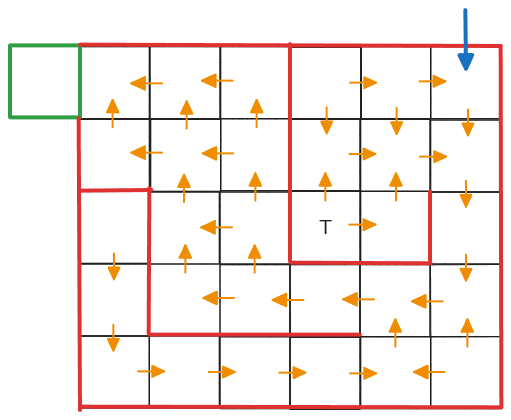
\includegraphics[width=0.50\linewidth]{labyrinthe07.png}
    \caption{Politique apprise pour \( p = 0{,}7 \)}
    \label{fig:pol_p07}
\end{figure}

\begin{figure}[H]
    \centering
    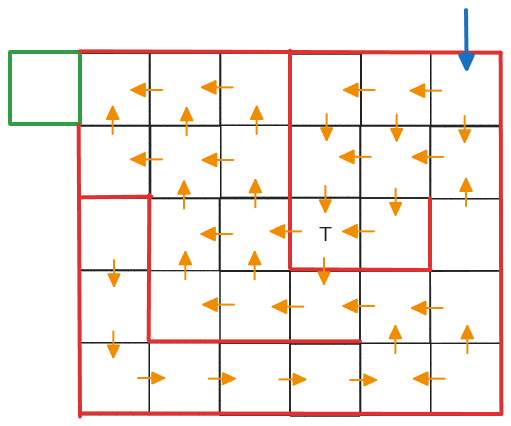
\includegraphics[width=0.50\linewidth]{labyrinthe09.png}
    \caption{Politique apprise pour \( p = 0{,}9 \)}
    \label{fig:pol_p09}
\end{figure}

Dans le cas \( p = 0{,}7 \), l’agent apprend à suivre un chemin direct vers la sortie principale, en évitant le téléporteur dans l’ensemble des états, y compris lorsqu’il se trouve sur la case du téléporteur. Cela indique que, pour cette valeur de \( p \), le passage par le téléporteur est systématiquement désavantageux.
À l’inverse, pour \( p = 0{,}9 \), on observe un basculement progressif de la stratégie : à partir d’une certaine distance par rapport à la sortie, l’agent apprend à rejoindre le téléporteur pour bénéficier de la probabilité de téléportation. Cette transition correspond aux seuils \( p^*(s) \) calculés au préalable, qui définissent dans chaque état si le téléporteur est avantageux ou non.

Ces résultats illustrent le fait que la politique optimale dépend fortement de la structure probabiliste de l’environnement, et que l’apprentissage permet de s’y adapter. La cohérence entre les politiques apprises et les seuils théoriques confirme le bon comportement de l’algorithme dans ce cadre.



Pour différentes valeurs de \( p \), l’algorithme converge vers des stratégies qui exploitent ou non le téléporteur, selon qu’il est avantageux ou non d’y passer. Ces choix d’actions sont conformes aux prédictions issues du calcul des seuils \( p^*(s) \) : on observe que pour \( p < p^*(s) \), l’agent privilégie le chemin direct, tandis que pour \( p > p^*(s) \), il choisit d’atteindre le téléporteur. Cette correspondance valide à la fois la dynamique d’apprentissage et les résultats théoriques présentés précédemment.

\subsection{Apprentissage dans un environnement complexe}

Dans cette dernière expérience, nous considérons un environnement plus complexe que le précédent : un labyrinthe de taille \(10 \times 10\), comprenant des cases à récompense positive (affichées en vert clair, valeur \(+5\)), des cases à récompense négative (en rouge, valeur \(−5\)), ainsi qu’une case spéciale agissant comme un téléporteur (en violet), ramenant systématiquement l’agent au point de départ (situé en bas à gauche, affiché en bleu clair). L’objectif est d’atteindre la sortie, représentée en vert foncé, et placée en haut à droite de la grille.


\begin{figure}[H]
    \centering
    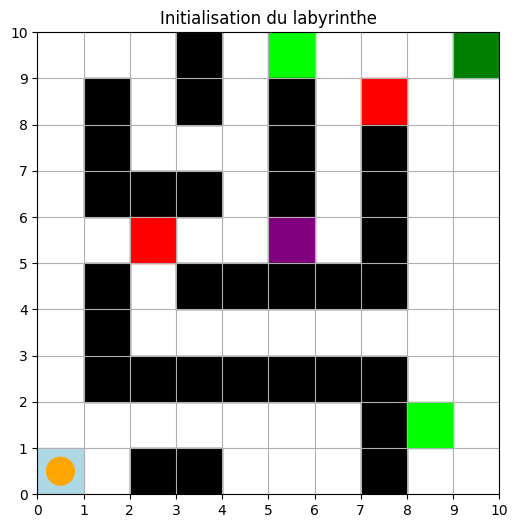
\includegraphics[width=0.5\textwidth]{INI.png}
    \caption{Labyrinthe \(10 \times 10\) utilisé pour l'entraînement.}
\end{figure}

L'algorithme de Q-learning est appliqué sans modification structurelle, en conservant les mêmes paramètres que précédemment : taux de réduction de l'exploration \(\varepsilon_n = \frac{1}{1+n}\), taux d’apprentissage \(\alpha_n = \frac{1}{1 + N(s,a)}\), et facteur d’actualisation \(\gamma = 0{,}95\). Le nombre d’épisodes est porté à 10\,000 afin de permettre une convergence satisfaisante dans cet environnement plus complexe.

Nous avons sélectionné 3 trajectoire à afficher au cours de l’algorithme pour illustrer l'apprentissage: au début (épisode 0), à mi-parcours (épisode 5\,000), et à la fin (épisode 10\,000). La figure ci-dessous montre l’évolution progressive de la stratégie de l’agent.

\begin{figure}[H]
    \centering
    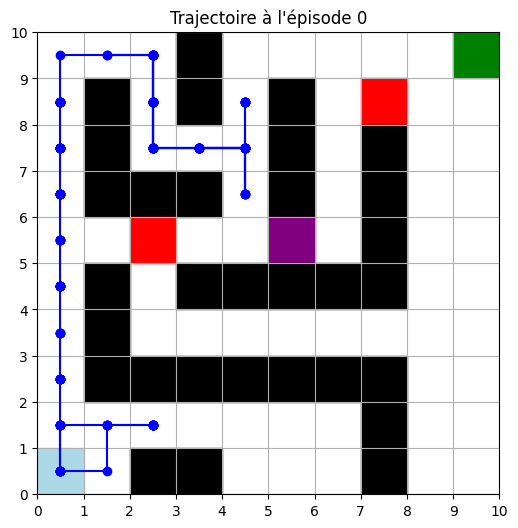
\includegraphics[width=0.32\textwidth]{TRAJECTOIRE 0.png}
    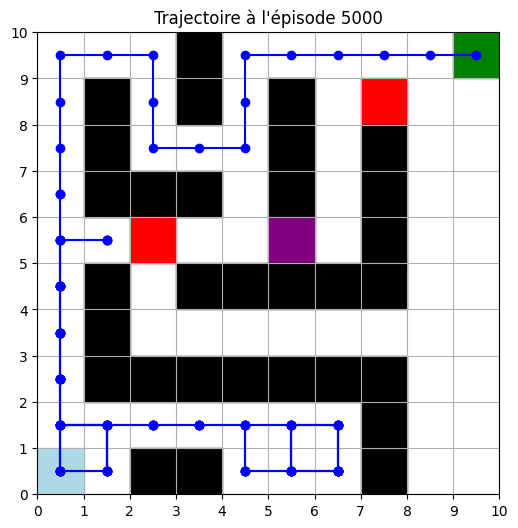
\includegraphics[width=0.32\textwidth]{TRAJECTOIRE5K.png}
    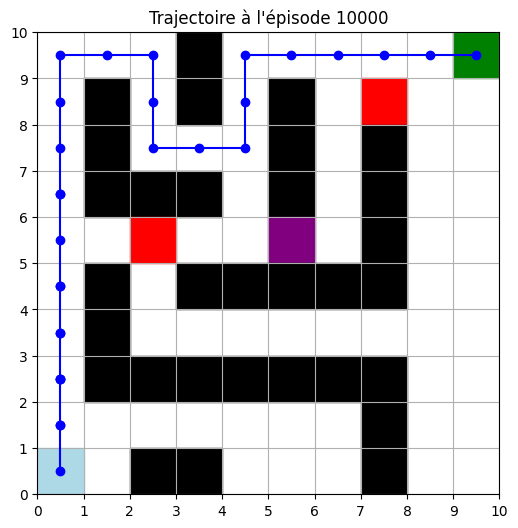
\includegraphics[width=0.32\textwidth]{TRAJECTOIREPARFAIT.png}
    \caption{Trajectoires de l’agent à différents moments de l’apprentissage : épisode 0 (gauche), épisode 5\,000 (centre), épisode 10\,000 (droite).}
\end{figure}

Au tout début de l'apprentissage (épisode 0), l’agent se déplace de manière aléatoire, sans structure apparente. Il effectue de nombreux allers-retours et tourne en rond dans certaines zones du labyrinthe, sans jamais atteindre la sortie.

À mi-parcours (épisode 5\,000), une stratégie globale commence à se dessiner : l’agent parvient à atteindre la sortie, mais emprunte encore un chemin sous-optimal, s’arrêtant inutilement sur certaines cases intermédiaires ou explorant des zones sans intérêt avant de rejoindre l’arrivée.

À la fin de l’apprentissage (épisode 10\,000), la politique apprise est optimale : l’agent atteint la sortie rapidement et sans détour, en suivant un chemin direct, tout en évitant les pièges, la case téléporteur et les zones sans utilité.


Cette expérience illustre à la fois la capacité du Q-learning à converger vers une stratégie efficace dans un environnement complexe, et le coût en nombre d’épisodes nécessaire pour y parvenir.


\subsection{Coûts et limites du Q-learning}

L’algorithme de Q-learning appliqué dans ce labyrinthe \(10 \times 10\) a permis, après 10\,000 épisodes, d’obtenir une politique optimale menant systématiquement à la sortie sans détour. Le temps total d’apprentissage observé a été d’environ 20 secondes pour un total d’environ 800\,000 actions effectuées.

En termes de complexité, le Q-learning présente l’avantage d’une mise en œuvre simple, ne nécessitant ni modèle de transition ni connaissance de la fonction de récompense. Toutefois, cette simplicité s’accompagne d’un coût d’apprentissage important, en particulier dans des environnements de grande taille ou fortement stochastiques. L’algorithme explore l’environnement par essais-erreurs et nécessite de nombreuses interactions pour converger, ce qui peut poser des problèmes dans certains contextes où l’échantillonnage est coûteux ou limité.

Par ailleurs, nous avons été confrontés à des situations où la politique semblait optimale à un certain moment de l’apprentissage, avant de se détériorer légèrement par la suite. Ce type de comportement est classique avec le Q-learning . Tant que les Q-valeurs continuent d’être mises à jour, même lentement, l’algorithme peut renforcer des trajectoires sous-optimales si celles-ci conduisent à des gains proches de ceux de la stratégie optimale. Cela empêche une stabilisation complète de la politique, malgré une convergence apparente.
.


Le Q-learning fonctionne bien dans certains cas, mais il a aussi plusieurs limites. Voici quelques-unes des principales difficultés qu’on peut rencontrer avec cette méthode :



\begin{itemize}
    \item \textbf{Convergence parfois lente} : dans les environnements de grande taille ou lorsque les récompenses sont différées, il faut souvent un grand nombre d’épisodes pour obtenir une stratégie satisfaisante.

    \item \textbf{Variabilité des Q-valeurs} : même après convergence apparente, les Q-valeurs peuvent continuer à évoluer, notamment si l’algorithme explore encore certaines parties de l’espace d’états.

    \item \textbf{Politique instable} : une politique qui semblait correcte peut se dégrader légèrement par la suite, surtout si l’agent continue à renforcer des actions sous-optimales.

    \item \textbf{Paramètres sensibles} : le choix de \(\alpha_n\), \(\gamma\) et surtout de \(\varepsilon_n\) influence fortement le comportement de l’algorithme. Des mauvais réglages peuvent empêcher la convergence ou ralentir l’apprentissage.

    \item \textbf{Pas adapté aux espaces continus} : dans un cadre continu, il faut recourir à des méthodes d’approximation. Le Q-learning tabulaire n’est plus utilisable directement.

    \item \textbf{Exploration difficile à calibrer} : si \(\varepsilon_n\) décroît trop vite, l’agent n’explore pas assez ; s’il reste trop élevé, il continue à prendre des décisions aléatoires même quand la politique est presque stable.
\end{itemize}


Au final, le Q-learning reste une méthode simple et efficace dans certaines situations, mais son comportement peut beaucoup varier selon l’environnement et la façon dont l’agent explore pendant l’apprentissage.


\section*{Conclusion}

Ce projet nous a permis d’explorer plusieurs aspects des processus décisionnels de Markov, aussi bien d’un point de vue théorique que pratique. Après avoir formalisé les notions de base (espaces d’états, politiques, fonctions de valeur, critères d’évaluation), nous avons appliqué ces outils à des environnements concrets sous forme de labyrinthes.

La première partie du travail a consisté à étudier différentes résolutions analytiques dans des cadres déterministes et probabilistes, avec ou sans horizon fini. Ces résultats nous ont servi de référence pour valider ensuite les politiques apprises par Q-learning.

Dans la deuxième partie, nous avons mis en œuvre l’algorithme de Q-learning dans plusieurs environnements, de difficulté croissante. L’apprentissage s’est montré efficace pour retrouver les politiques attendues dans les cas simples. Dans les environnements plus complexes, l’algorithme a fini par converger vers des stratégies pertinentes, à condition d’avoir suffisamment d’épisodes d’entraînement et des paramètres bien choisis.

Cela nous a permis de mieux comprendre comment le Q-learning fonctionne en pratique : ses points forts (autonomie, absence de modèle) mais aussi ses limites (coût en temps, instabilité possible, sensibilité aux réglages). Nous avons également constaté que même dans des environnements discrets et  petits, l’apprentissage peut être long et fragile.

Une suite logique de ce travail pourrait consister à tester des variantes plus robustes du Q-learning, notamment les versions utilisant des réseaux de neurones (DQN), ou des méthodes plus avancées comme l’acteur-critique. On pourrait aussi s’intéresser à des environnements partiellement observables ou à des tâches en continu, où le Q-learning  ne suffit plus.

Enfin, ce type d’approche pourrait être adapté à des cas d’usage plus concrets, par exemple dans des applications de robotique, de planification ou de jeu, où les décisions doivent être prises dans des environnements complexes avec des objectifs multiples. Ce serait un prolongement pour mieux relier ces méthodes à des situations réelles.


\end{document}